During the development of the project, the team encountered a number of challenges. The primary issue was translating the car's behaviour from the simulation into the actual environment. The subsequent challenges required significant time and effort to address, resulting in unanticipated delays in the project timeline.
\newline
Before setting up the Slam Toolbox and while working on the M2P node, we wanted to validate the driving behaviour to a target point in the real world. We found that ROS and Gazebo use different coordinate systems which resulted in correct calculations in the simulations but incorrect calculations in the real world tests. This was due to the odometry and the target points were not reaching the same point. This problem was overcome by writing a transformation node that used a static transform publisher with modified orientations for the car platform frame, but still used the default values for the simulation by simply passing the target point to the correct frame. This would translate between both coordinate systems depending on the context of use.\\
Furthermore, during a debugging session, it became evident that there was an additional discrepancy between the simulation and the actual scenario. In reality, the racecar would come to a halt just before the range for the M2P node was able to consider a point to be reached. This was due to the velocity of the drive message for the racecar being too small to enable forward movement. To address this issue, a minimum velocity was implemented and the handling of target points in the M2P node was adjusted slightly. In earlier iterations the MoveToPoint node was maintaining a stack of points and working it off by arriving at the current target point and setting its next target point by popping the stack. In the current iteration the MoveToPoint node maintains only one target point.
\newline
In addition, the team encountered issues with the transform tree and working with rosbags. These issues have expressed themselves as a significant drift in odometry and inaccuracies in the sensor data lookup. Consequently, self-localisation and mapping appeared unfeasible in a real-world setting. However, following a system update on the racecar, the issue was resolved, and the rosbags were able to deliver reasonable maps. Figure \ref{fig:map} illustrates a broken map prior to the update.

\begin{figure}[htp]
	\vskip 0.2in
	\begin{center}
		\centerline{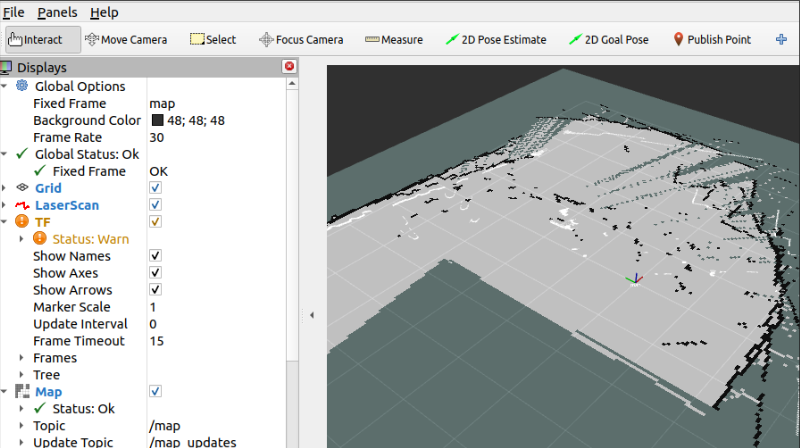
\includegraphics[width=\columnwidth]{mapping.png}}
		\caption{Screenshot of the RViz application, showing the visualisation of the faulty transform when replaying a rosbag.}
		\label{fig:map}
	\end{center}
	\vskip -0.2in
\end{figure}